\subsection{Startup behaviour of the Ozone generator}
\label{sec:ozone}

These are the first experiments conducted using the setup described in
Section~\ref{sec:ozone-setup}. The first goal was to see whether our
setup produced any Ozone at all, i.\,e.\ whether the Silica gel became
permeable for Ozone or not. In a second step we researched the startup
behaviour of our system, as it is important to know the startup time
necessary before our generator reaches a stable Ozone output. Lastly
we checked the influence of the Pen-Ray lamp power on the Ozone
concentration. Using this setup it was impossible to test the
filtering effects on \ch{NO2} produced by the generator. Since the
concentration should be around the \ch{NO_x} concentration in ambient
lab air, it should be no more than a few \si{ppb}. This is far below
the detection limit of a longpath DOAS instrument with a pathlength of
\SI{10}{\centi\meter}. 

Turning on the generator very quickly produced an Ozone signal. Thus
we started a more in depth analysis. Turning of the generator for
about a week and then taking measurements right after turning it on,
we yielded Figure~\ref{fig:long-stop}. As can be seen the generator
takes about \SI{35}{\minute} before it reaches its stable plateau of
around \SI{250}{ppb} Ozone. During this experiment the flow was
constantly set to $\Phi_{\ch{O_3}} = \SI{0.03}{\liter\per\minute}$. It
stands to argue that the startup time could be shortened by increasing
the flow and returning to a lower value later, when the actual \ch{NO_x}
measurements are performed. Furthermore the Hg-lamp power supply was
set to \SI{10}{\milli\ampere}.

\begin{figure}[htbp]
  \centering
  \begin{tikzpicture}
    \begin{axis}[
      xlabel={Time [\si{\hour}]},
      ylabel={c(\ch{O3}) [ppb]},
      no markers,
      xmin=0,
      xmax=2,
      ]
      \addplot table [col sep=comma] {images/Anschaltkurve2.csv};
    \end{axis}
  \end{tikzpicture}
  \caption{Evolution of Ozone after a long full stop of the
    generator.}
  \label{fig:long-stop}
\end{figure}

Next we were interested in the short term startup behaviour of the
system. We stopped the generator after it had reached a stable level
and restarted it after a fixed time period. The result can be found in
Figure~\ref{fig:multiple-stop}. Since the time resolution of the DOAS
instrument is rather coarse the only safe statement is, that even
after a \SI{4}{\hour} stop the concentration climbed back up to around
\SI{200}{ppb} after \SI{5}{\minute}. So it stands to reason, that if
the device is used regularly the a prolonged startup time should not
be an issue, even if one sticks to the constant flow of
$\Phi_{\ch{O3}} = \SI{0.03}{\liter\per\minute}$. As compared to the
Ozone level in Figure~\ref{fig:long-stop}, the plateau seems to lie
slightly lower in this second experiment. The reason for this lies
most probably in outer conditions such as temperature in the
laboratory, which changed rather drastically from day to day, as the
experiments were conducted in November and December.

\begin{figure}[htbp]
  \centering
  \begin{tikzpicture}
    \begin{axis}[
      xlabel={Time [\si{\minute}]},
      ylabel={c(\ch{O3}) [ppb]},
      legend entries={\nfrac 1/2\si{\hour}, \SI{1}{\hour}, \SI{2}{\hour},
        \SI{4}{\hour}},
      no markers,
      legend pos=south east,
      xmin=0,
      xmax=10,
      ]
      \addplot table [col sep=comma] {images/Multiple-stop.csv};
      \addplot table [col sep=comma,y=1h] {images/Multiple-stop.csv};
      \addplot table [col sep=comma,y=2h] {images/Multiple-stop.csv};
      \addplot table [col sep=comma,y=4h] {images/Multiple-stop.csv};
    \end{axis}
  \end{tikzpicture}
  \caption{Evolution of the Ozone concentration after a full stop of the
    generator.}
  \label{fig:multiple-stop}
\end{figure}

\begin{figure}[htbp]
  \centering
  \begin{tikzpicture}
    \begin{axis}[
      xlabel={Time [\si{\minute}]},
      ylabel={c(\ch{O3}) [ppb]},
      no markers,
      xmin=0,
      xmax=45,
      ]
      \addplot table [col sep=comma] {images/2015-12-02-current2.csv};
    \end{axis}
  \end{tikzpicture}
  \caption{Ozone level dependence on current of Hg-lamp. The steep
    flank occured after a change of the current from
    \SI{10}{\milli\ampere} to \SI{17}{\milli\ampere}.}
  \label{fig:lamp}
\end{figure}

After having analyzed the startup procedure, we wanted to at least get
the qualitative influence of the power supply current of the Pen-Ray
lamp on the Ozone concentration. Beforehand it was not clear whether a
higher current would increase or decrease the Ozone production rate,
as, as was described in Section~\ref{sec:theory-ozone}, we did not
know how a change in power would transform the power distribution on
the different Mercury lines. We recorded a timeseries while switching
between the two possible currents, \SI{10}{\milli\ampere} and
\SI{17}{\milli\ampere}, and yielded 
Figure~\ref{fig:lamp}. From this we see that we still work in a regime
where higher power leads to more Ozone. This is interesting to know,
however, since \SI{200}{ppb} is already more than enough Ozone for our
purposes, in the practical application we just used the current
which was easiest to set up\footnote{The currents of all used supplies
  lay in the same region.}.

\subsection{Silica gel influence on \ch{O3} and \ch{NO2} concentration}
\label{sec:silica}

In this experiment we wanted to deduce the influence of the Silica gel
filter, installed behind the Ozone generator, on the \ch{NO2} and
\ch{O3} concentration. For this we used the updated Cavity as
described in Section~\ref{sec:inclusion}. This setup was necessary as
the expected \ch{NO2} concentrations were so low, that they were
undetectable by a `longpath' instrument. The disadvantage of this
procedure lies in the fact, that the Ozone absorption in the visible
spectrum is much weaker than in the UV spectrum, such that we have to
accept higher uncertainties in the DOAS fit for this species. 

Additionally we did not measure the output of the generator directly,
as the Ozone concentration would have been so high as to damage the cavity's
main stream pump. Therefore we used a setup as depicted
in Figure~\ref{fig:ozone-flow-setup}, which used zero air cartridges at
both the sample air and the zero air input. This allowed us to dilute
the Ozone enriched air by mixing it with the `sample air', which was
then trace gas free and hence kept additional errors down.

We took three test series. For all of them the total flow was fixed to
$\Phi = \SI{2}{\liter\per\minute}$ and the Ozone flow $\Phi_{\ch{O3}}$
was varied between \num{0} and \SI{0.3}{\liter\per\minute}. The first
two series were recorded while increasing the Ozone flow, while the
last one was measured decreasingly. This was done to check for any
hysteresis effects in the Silica gel. Furthermore for the second
series the Silica gel filter had been removed. For each flow we waited
until the concentrations reached a stable level and then averaged over
several datapoints.

\begin{figure}[htbp]
  \centering
  
\includegraphics[width=0.35\textwidth]{ozone_setup.png}
  \caption{Ozone measurement setup}
  \label{fig:ozone-flow-setup}
\end{figure}

The result of our experiment can be found in
Figure~\ref{fig:o3-flow}. The left hand side describes the Ozone
concentration and we can see that hysteresis effects in the Silica gel
should are negligible. Within the errors thee ascending and descending
Ozone concentration coincide. The Ozone concentration measured without
Silica gel filter differs from the other two, however differently from
what we expected beforehand. The gel should adsorb some of the Ozone,
so it sounds reasonable that the absolute Ozone concentration
\emph{without} filter should be higher than the on \emph{with}
filter. However, as we can see, we measure exactly the opposite. 
\todo{why is ozone level without filter lower?}

Looking at the right hand side of Figure~\ref{fig:o3-flow}, we see the
strong influence of the Silica on the \ch{NO2} levels. With filter, we
have no \ch{NO2} signal, without it, we have concentrations that reach
up to \SI{14}{ppb}. So without filter we would introduce an error to
the \ch{NO_x} measurement that is in the order of magnitude of the
German rural background\todo{cite}. Utilizing the filter the error
introduced by the additional \ch{NO2} is negligible. We see that the
filter is a very effective tool to clean the generator air.

\begin{figure}[htbp]
  \centering
  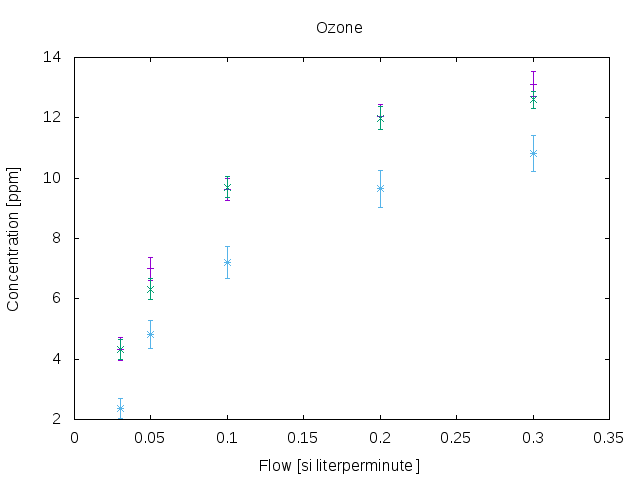
\includegraphics[width=0.45\textwidth]{O3.png}
  \hfill
  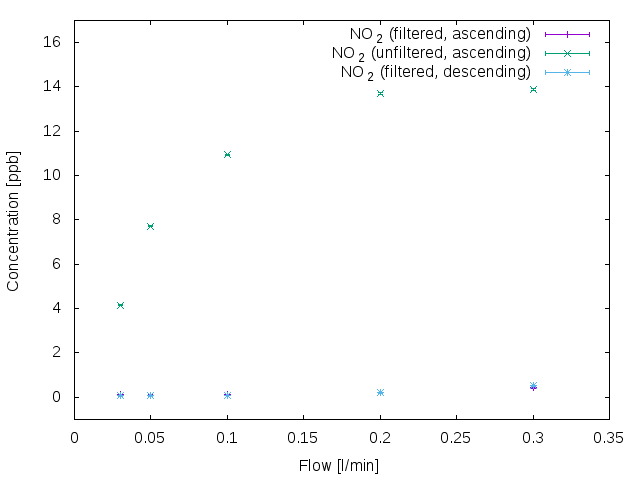
\includegraphics[width=0.45\textwidth]{NO2.png}
  \caption{\ch{O3} and \ch{NO2} concentration over generator flow.}
  \label{fig:o3-flow}
\end{figure}

%%% Local Variables: 
%%% mode: latex
%%% TeX-master: "../Bachelor"
%%% End: 
